\chapter{Marco teórico}
\label{ch:marco}

\section{Introducción del capítulo}

El análisis y procesamiento de señales constituye un elemento fundamental dentro de la ingeniería de computadores, particularmente en el diseño de sistemas digitales capaces de representar, transformar y transmitir información. En este contexto, la comprensión de los principios que rigen el comportamiento de las señales resulta indispensable para el desarrollo de técnicas que permitan su manipulación de manera controlada.

De manera análoga, cuando el tratamiento de señales se aborda dentro del desarrollo de soluciones en entornos computacionales específicos, surgen consideraciones adicionales que deben ser tomadas en cuenta para su correcta aplicación. Estas condiciones introducen nuevos elementos en el análisis, los cuales difieren de aquellos presentes en entornos de desarrollo más generales, haciendo necesario ampliar la base conceptual desde la cual se estudian estos procesos.

En el presente capítulo se establece el conjunto de fundamentos teóricos necesarios para comprender el tratamiento de señales, su transformación y las consideraciones asociadas a su implementación en sistemas digitales. A partir de esta base, se construye un marco conceptual que permite abordar de manera estructurada los elementos que intervienen en el desarrollo del problema de estudio.

\section{Mapa conceptual del marco teórico}

Con el fin de organizar de manera estructurada los conceptos desarrollados en este capítulo, se presenta el mapa conceptual mostrado en la Figura \ref{fig:mapa_conceptual}. Este permite visualizar la relación entre los distintos elementos teóricos y la progresión lógica bajo la cual serán abordados.

\begin{figure}[H]
\centering
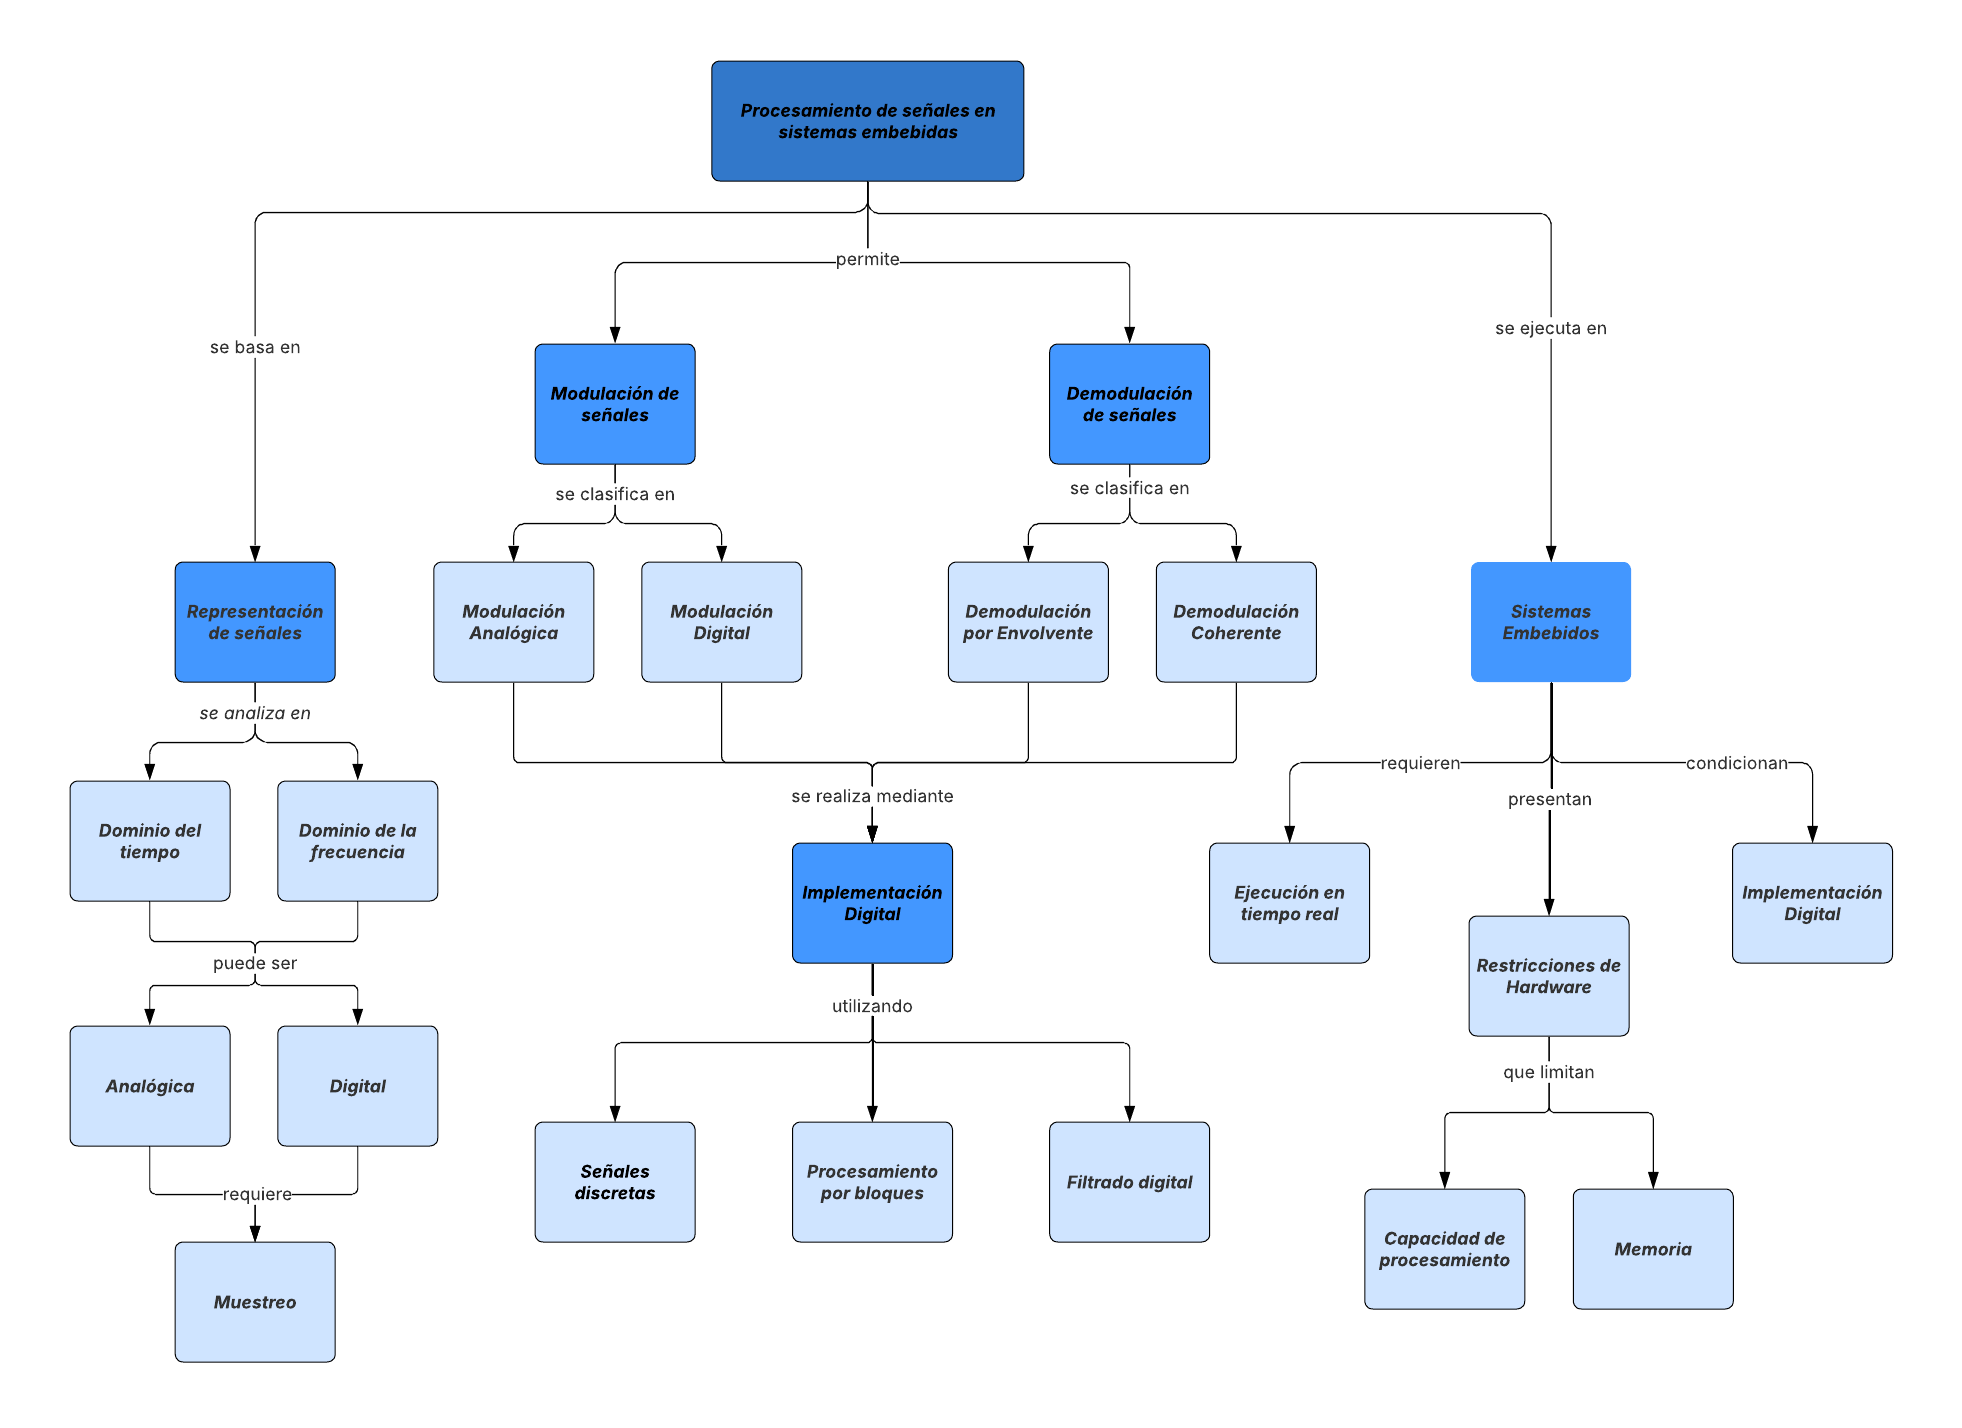
\includegraphics[width=0.9\linewidth]{../fig/mapaconceptual.png}
\caption{Mapa conceptual del marco teórico. Fuente: Elaboración Propia.}
\label{fig:mapa_conceptual}
\end{figure}

Tal como se observa en la Figura \ref{fig:mapa_conceptual}, el desarrollo conceptual se estructura a partir de los fundamentos de procesamiento de señales, donde se establecen las bases para la representación de señales en distintos dominios. A partir de esta base, se introduce el proceso de modulación, considerando tanto enfoques analógicos como digitales, seguido por los mecanismos asociados a la demodulación de dichas señales.

Posteriormente, se incorpora la etapa de implementación digital, en la cual se consideran aspectos relacionados con la representación discreta, el procesamiento por bloques y el filtrado digital. Finalmente, el marco conceptual se completa con el análisis de los sistemas embebidos, donde se integran las restricciones de hardware y los requerimientos de tiempo real. Esta secuencia establece una transición progresiva desde la caracterización de señales hasta su ejecución en entornos embebidos.



\section{Fundamentos de procesamiento de señales}

El procesamiento de señales se fundamenta en el estudio de las representaciones matemáticas de la información y en las operaciones que pueden realizarse sobre estas para su análisis y transformación. Según Oppenheim y Willsky, en la teoría de Señales y Sistemas, este campo aborda la caracterización, manipulación y extracción de información contenida en señales mediante modelos matemáticos formales \cite{oppenheim1997}. En el contexto de sistemas digitales, este estudio permite comprender cómo la información es modelada, manipulada y posteriormente utilizada dentro de distintos procesos computacionales.

\subsection{Definición de señal}

En este contexto, el concepto de señal constituye el punto de partida para el análisis, ya que permite formalizar la manera en que la información es representada dentro de un sistema.

De acuerdo con \cite{oppenheim1997}, una señal puede entenderse como una función que describe la variación de una magnitud en relación con una o más variables independientes. En la mayoría de los sistemas de interés en ingeniería, dicha variable corresponde al tiempo, lo que permite representar la evolución de la información dentro de un sistema.

Una señal continua puede representarse de forma general como:

\begin{equation}
x(t)
\end{equation}

donde $x$ denota la señal y $t$ representa la variable independiente asociada al tiempo. Esta formulación permite modelar fenómenos físicos y procesos de información que varían de manera continua, tales como señales eléctricas o acústicas presentes en sistemas electrónicos \cite{oppenheim1997}.

Por otra parte, cuando la señal es tratada en sistemas digitales, su representación se realiza de forma discreta mediante una secuencia de valores definidos en instantes específicos. En este caso, la señal puede expresarse como:

\begin{equation}
x[n]
\end{equation}

donde $n$ es un índice entero que identifica cada muestra dentro de la secuencia. Esta representación es fundamental en el procesamiento digital, ya que permite manipular la señal mediante algoritmos y estructuras propias de sistemas computacionales \cite{oppenheim1997}.

Con el fin de complementar la representación matemática de las señales, es necesario considerar las magnitudes fundamentales que permiten caracterizar su comportamiento. En la Figura \ref{fig:parametros_senal}, se ilustran los principales parámetros asociados a una señal senoidal.

\begin{figure}[H]
\centering
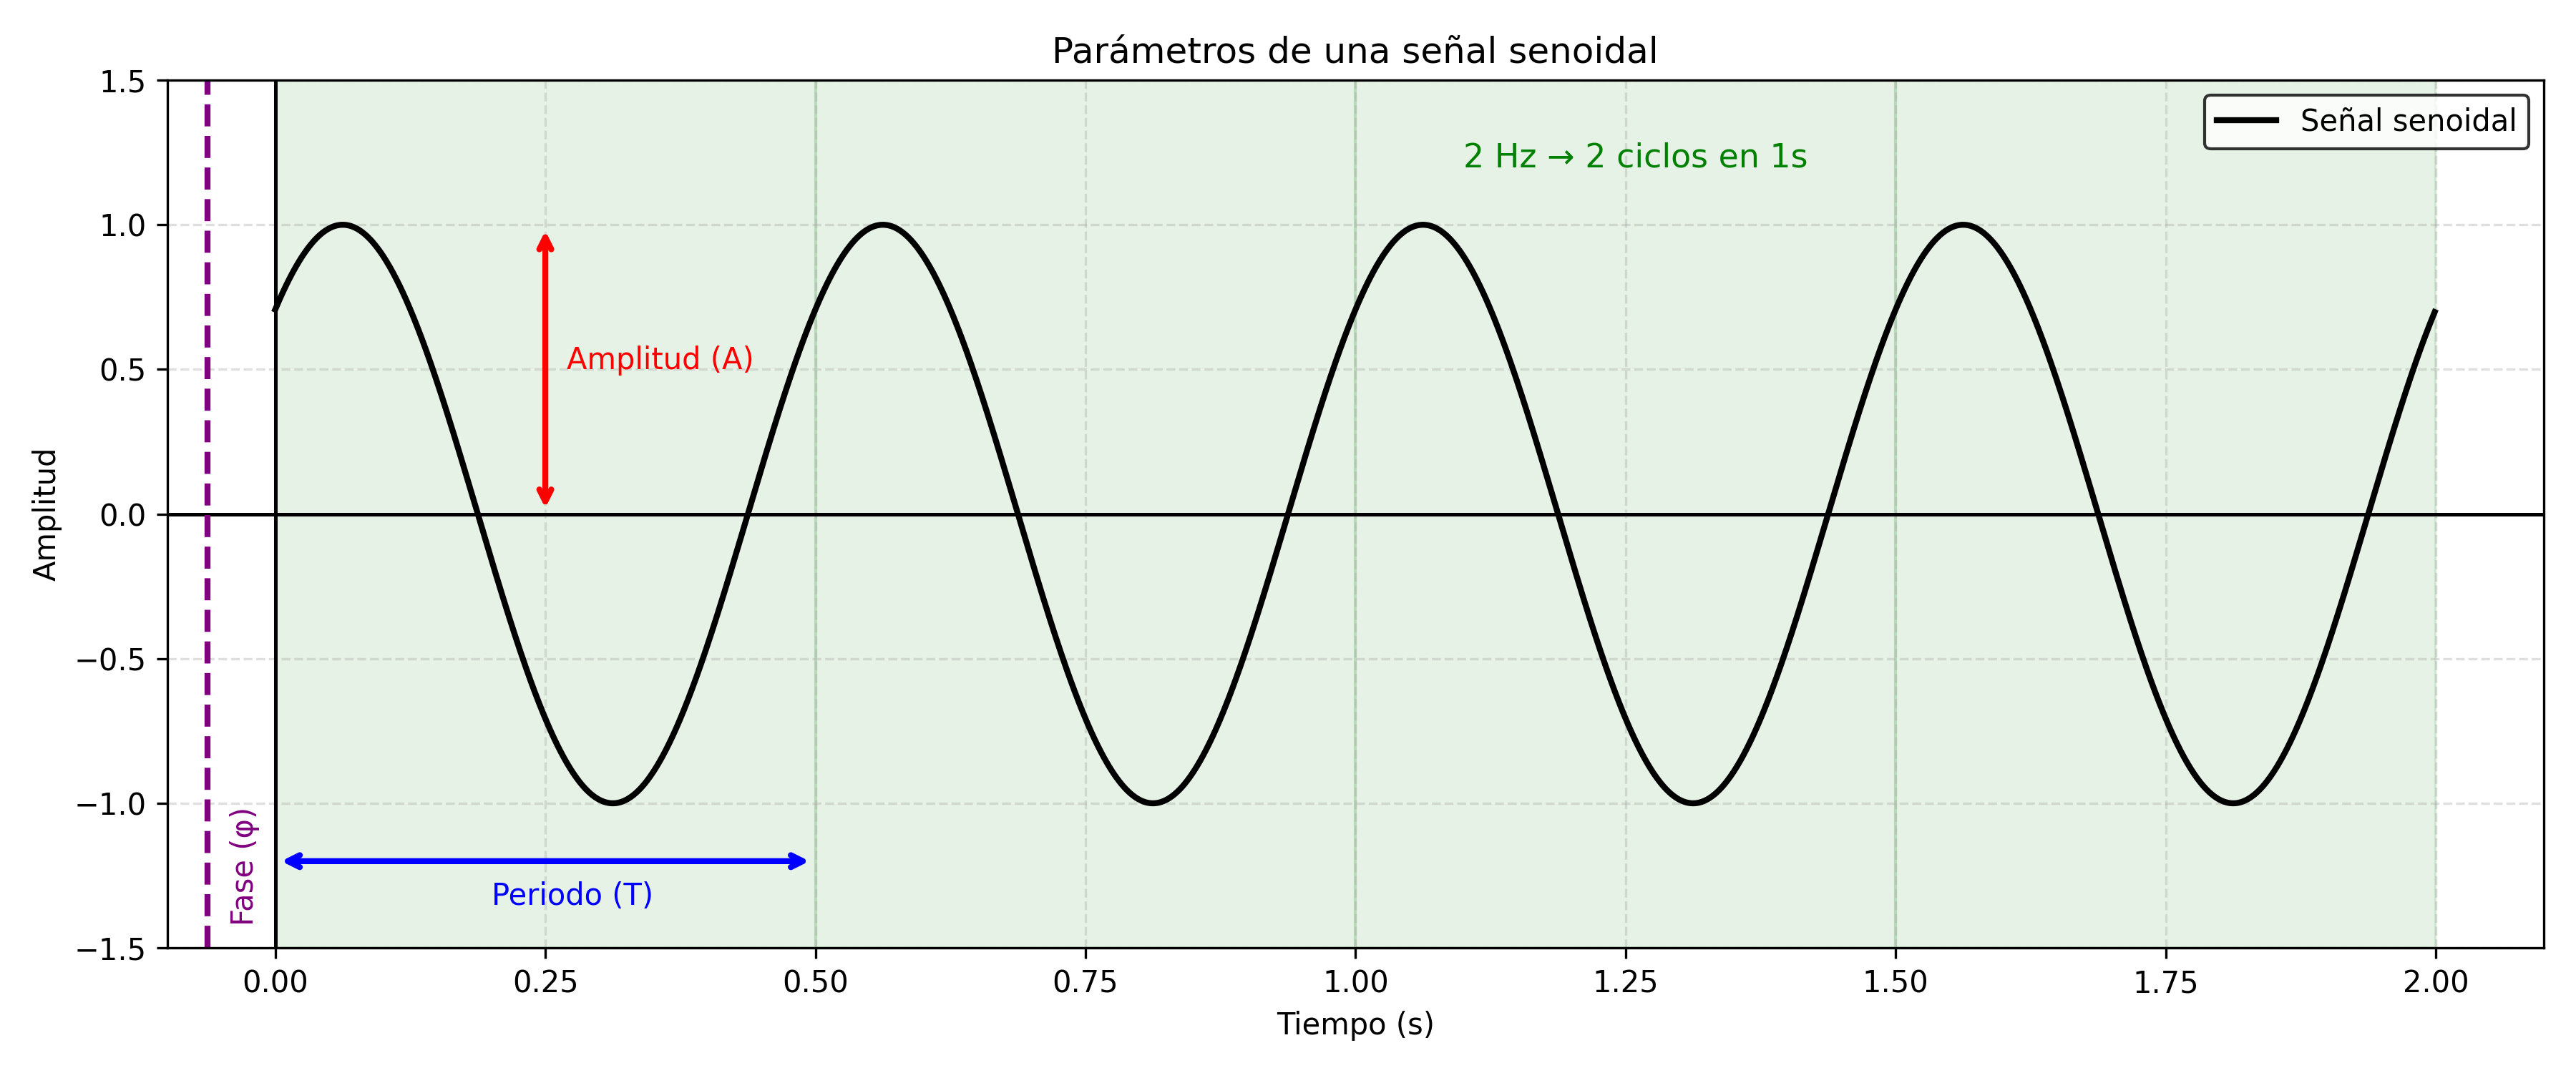
\includegraphics[width=0.9\linewidth]{../fig/onda_senoidal.png}
\caption{Parámetros fundamentales de una señal senoidal. Fuente: Elaboración Propia.}
\label{fig:parametros_senal}
\end{figure}

Tal como se muestra en la Figura \ref{fig:parametros_senal}, la amplitud corresponde al valor máximo que alcanza la señal respecto a su nivel de referencia, representando la intensidad de la magnitud descrita. El periodo, denotado como $T$, define el intervalo de tiempo en el cual la señal completa un ciclo. La frecuencia, representada como $f$, indica el número de ciclos por unidad de tiempo  \cite{lathi2009modern} y se relaciona con el periodo según:

\begin{equation}
f = \frac{1}{T}
\label{eq:frecuencia_periodo}
\end{equation}

Adicionalmente, la fase describe el desplazamiento relativo de la señal respecto a un origen de referencia en el tiempo, permitiendo identificar la posición inicial de la señal dentro de su ciclo. Estos parámetros constituyen la base para la descripción y análisis de señales en ingeniería, y serán utilizados de forma recurrente en el desarrollo de los procesos de modulación y demodulación abordados en las secciones posteriores.


\subsection{Señales en el dominio del tiempo y la frecuencia}

A partir de la representación de una señal, su análisis puede abordarse desde distintas perspectivas dependiendo de la información que se desee obtener. En este sentido, una misma señal puede ser descrita tanto en el dominio del tiempo como en el dominio de la frecuencia, lo que permite caracterizar su comportamiento desde enfoques complementarios.

En el dominio del tiempo, la señal se representa directamente como una función de la variable independiente, lo que permite observar su evolución a lo largo del tiempo. Esta representación resulta adecuada para analizar propiedades como la amplitud y la forma de la señal.

Por otra parte, el dominio de la frecuencia permite describir la señal en términos de las componentes espectrales que la conforman. De acuerdo con \cite{oppenheim1997}, cualquier señal puede expresarse como una combinación de componentes sinusoidales de distintas frecuencias.

La relación entre ambas representaciones se ilustra en la Figura \ref{fig:tiempo_frecuencia}. En el dominio del tiempo se observa una señal compuesta, cuya forma no permite identificar de manera directa las componentes que la originan. Sin embargo, al analizarla en el dominio de la frecuencia, se evidencian claramente las componentes sinusoidales presentes, representadas mediante picos en frecuencias específicas.

\begin{figure}[H]
\centering

\includegraphics[width=0.9\linewidth]{tiempo_frecuencia.png}
\caption{Representación de una señal compuesta en el dominio del tiempo y su correspondiente espectro de magnitud. Fuente: Elaboración Propia.}
\label{fig:tiempo_frecuencia}
\end{figure}

Según \cite{oppenheim1997}, la relación entre el dominio del tiempo y la frecuencia puede describirse mediante la Transformada de Fourier:

\begin{equation}
X(f) = \int_{-\infty}^{\infty} x(t)e^{-j2\pi ft} , dt
\label{eq:fourier}
\end{equation}

donde $X(f)$ representa la transformada de la señal $x(t)$, $f$ corresponde a la frecuencia y $j$ es la unidad imaginaria. Esta transformación permite describir cómo se distribuyen las componentes de la señal en función de la frecuencia.

La comprensión de estas dos representaciones resulta fundamental para el análisis de señales, ya que permite abordar tanto su comportamiento temporal como su composición espectral. A partir de esta base, es posible establecer una clasificación de las señales según la naturaleza de su representación.

\subsection{Señales analógicas y digitales}

Tal como se presenta en la Figura \ref{fig:mapa_conceptual}, una vez establecidas las formas de representación de las señales, resulta necesario considerar su clasificación según la naturaleza de los valores que adoptan y la forma en que son tratadas dentro de un sistema.

Según Lathi, en el estudio de sistemas de comunicación modernos, una señal analógica se caracteriza por tomar valores continuos tanto en el tiempo como en amplitud \cite{lathi2009modern}. Este tipo de señal es común en fenómenos físicos, donde las magnitudes varían de manera continua, como es el caso de señales eléctricas, acústicas o electromagnéticas.

Por otra parte, una señal digital se define por tomar valores discretos en el tiempo y, en la mayoría de los casos, también en amplitud. Este tipo de representación es propia de los sistemas digitales, donde la información es tratada como una secuencia de valores que pueden ser almacenados, procesados y transmitidos mediante estructuras y algoritmos computacionales \cite{proakis2001digital}. En aplicaciones prácticas, este tipo de señales es ampliamente utilizado en sistemas de comunicación y procesamiento implementados en plataformas digitales \cite{stm32_comm}.

\subsection{Muestreo y discretización}

El tratamiento de señales en sistemas digitales requiere establecer un mecanismo que permita representar señales continuas mediante una forma discreta. En \cite{oppenheim1997}, el muestreo se define como el proceso mediante el cual una señal continua en el tiempo es evaluada en instantes específicos, generando una secuencia de valores que puede ser procesada digitalmente.

A partir de este proceso, la señal discreta puede expresarse como:

\begin{equation}
x[n] = x(nT_s)
\end{equation}

donde $T_s$ representa el período de muestreo y $n$ es un índice entero que identifica cada muestra. La frecuencia de muestreo asociada se define de forma análoga a la relación entre frecuencia y periodo presentada en la Ecuación \ref{eq:frecuencia_periodo}, obteniéndose:

\begin{equation}
f_s = \frac{1}{T_s}
\end{equation}

El proceso de muestreo se ilustra en la Figura \ref{fig:muestreo}, donde se observa una señal continua junto con los valores discretos obtenidos al evaluarla en instantes uniformemente espaciados. En esta representación, las muestras corresponden a los valores de la señal en dichos instantes, evidenciando cómo la señal continua es representada mediante un conjunto finito de puntos.

\begin{figure}[H]
\centering

\includegraphics[width=0.9\linewidth]{muestreo.png}
\caption{Ejemplo de muestreo de una señal continua. Fuente: Elaboración Propia.}
\label{fig:muestreo}
\end{figure}

Para que la señal original pueda ser representada adecuadamente a partir de sus muestras, es necesario que la frecuencia de muestreo cumpla con ciertos criterios. Según Shannon, en la teoría de comunicaciones, si se desea que una señal pueda ser reconstruida sin pérdida de información, la frecuencia de muestreo debe ser al menos el doble de la máxima frecuencia presente en la señal \cite{shannon1949}. Este resultado es conocido como el teorema de Nyquist-Shannon.

De manera formal, esta condición puede expresarse como:

\begin{equation}
f_s \geq 2f_{max}
\label{eq:nyquist}
\end{equation}

donde $f_s$ corresponde a la frecuencia de muestreo y $f_{max}$ representa la máxima frecuencia presente en la señal. El cumplimiento de esta condición garantiza que las componentes frecuenciales de la señal puedan ser representadas sin ambigüedad en el dominio discreto.

El análisis de estas condiciones resulta fundamental para comprender cómo el contenido de una señal se preserva durante su representación digital, estableciendo una relación directa con la forma en que puede ser caracterizado en términos de sus componentes en frecuencia.


\subsection{Representación espectral}

La representación de una señal en el dominio de la frecuencia permite describirla en términos de sus componentes espectrales, proporcionando una perspectiva basada en su contenido frecuencial. Tal como se ilustra en la Figura \ref{fig:tiempo_frecuencia}, el espectro de una señal representa la distribución de dichas componentes en función de la frecuencia.

A partir de la relación entre el dominio del tiempo y el dominio de la frecuencia, expresada previamente mediante la Transformada de Fourier en la ecuación \eqref{eq:fourier}, resulta posible identificar las frecuencias presentes en una señal y analizar cómo se distribuyen en términos de amplitud o energía, lo cual es fundamental para su caracterización en sistemas de procesamiento \cite{lathi2009modern}.

El espectro de magnitud, en particular, permite visualizar la intensidad de las componentes presentes en la señal, facilitando la identificación de frecuencias dominantes y estableciendo una base para su manipulación en función de sus características frecuenciales, como ocurre en procesos de modulación.



\section{Modulación de señales}

La modulación constituye uno de los procesos fundamentales en el tratamiento de señales dentro de los sistemas de comunicación. Su estudio permite comprender cómo una señal puede ser transformada para cumplir con los requisitos impuestos por un medio de transmisión, estableciendo así un vínculo entre la representación de la señal y su capacidad de propagación. En este sentido, la modulación se aborda como un mecanismo de transformación controlada de señales, cuyo análisis resulta esencial para el desarrollo de técnicas de transmisión eficientes.

\subsection{Definición de modulación}

El concepto de modulación ha sido abordado desde distintas perspectivas en la literatura. Según Haykin, en el contexto de los sistemas de comunicación, la modulación se define como el proceso mediante el cual una señal de información altera una propiedad de una señal de mayor frecuencia, con el propósito de facilitar su transmisión \cite{haykin2001communication}. Por su parte, Proakis y Salehi plantean que la modulación no solo implica dicha interacción entre señales, sino que además permite trasladar el contenido de información hacia bandas de frecuencia específicas, favoreciendo la multiplexación y el aprovechamiento eficiente del espectro disponible \cite{proakis2007digital}.

Ambas definiciones coinciden en que la modulación implica una transformación de la señal original y, de manera complementaria, permiten entender este proceso tanto desde la interacción entre señales como desde su función dentro del sistema de comunicación. En conjunto, estas perspectivas establecen que la modulación no solo modifica características de una señal, sino que también responde a condiciones específicas impuestas por el medio de transmisión.

En términos generales, la modulación puede interpretarse como un proceso mediante el cual una señal de información es representada a través de otra señal, modificando parámetros fundamentales como la amplitud, la frecuencia o la fase, lo que permite su adecuación a condiciones específicas de transmisión sin alterar el contenido esencial de la información.

\subsubsection{Señal mensaje y señal portadora}

Una vez definido el concepto de modulación, resulta necesario considerar las señales que intervienen en este proceso. En términos generales, la modulación se fundamenta en la interacción entre una señal mensaje y una señal portadora, cuya relación permite representar y trasladar la información dentro de un sistema de comunicación.

La señal mensaje, denotada como $m(t)$, corresponde a la señal que contiene la información que se desea transmitir. Su naturaleza depende del sistema considerado, ya que puede representar distintas magnitudes de interés, tales como audio, voz, datos o cualquier otra forma de información susceptible de ser transportada. En muchos casos, esta señal presenta componentes de baja frecuencia en comparación con la portadora, por lo que actúa como la fuente de información que será incorporada al proceso de modulación \cite{lathi2009modern}.

Por su parte, la señal portadora corresponde a una señal periódica de mayor frecuencia que actúa como soporte para la transmisión de la información contenida en la señal mensaje. Según \cite{lathi2009modern}, en los sistemas de comunicación modernos, esta señal suele representarse mediante una función sinusoidal, debido a que su comportamiento matemático facilita el análisis de los procesos de modulación. De forma general, la portadora puede expresarse como:

\begin{equation}
c(t) = A_c \cos(2\pi f_c t)
\label{eq:carrier}
\end{equation}

donde $A_c$ corresponde a la amplitud de la portadora y $f_c$ a su frecuencia.

La interacción entre $m(t)$ y $c(t)$ da lugar a la señal modulada, en la cual la información de la señal mensaje queda contenida en alguna de las propiedades de la portadora. En este sentido, la señal mensaje define el contenido informativo, mientras que la portadora establece la base sobre la cual dicho contenido puede ser transportado. Esta distinción resulta esencial para comprender las distintas técnicas de modulación desarrolladas en sistemas de comunicación.

\subsection{Modulación analógica}

La modulación analógica se caracteriza por operar sobre señales cuyo comportamiento es continuo en el tiempo y en amplitud. En este tipo de modulación, la señal mensaje modifica de manera proporcional alguna propiedad de la señal portadora, generando una señal modulada que conserva la naturaleza continua de la información original.

Según \cite{haykin2001communication}, las principales variantes de modulación analógica corresponden a la modificación de la amplitud, la frecuencia o la fase de la portadora. Por su parte, \cite{lathi2009modern} destaca que estas técnicas surgen como respuesta a diferentes requerimientos del canal, tales como la eficiencia espectral o la robustez frente al ruido.

Esta clasificación permite entender que la modulación analógica no corresponde a una única técnica, sino a un conjunto de métodos que comparten un principio común, la representación continua de la información mediante la alteración de parámetros de una señal portadora.

De acuerdo con \cite{haykin2001communication}, en función del parámetro de la señal portadora que es modificado, es posible distinguir las siguientes técnicas principales:

\textbf{AM:} En la modulación en amplitud, la amplitud de la señal portadora varía en función de la señal mensaje, manteniendo constantes su frecuencia y fase.

\textbf{FM:} En la modulación en frecuencia, la frecuencia instantánea de la señal portadora se modifica en función de la señal de información, mientras que su amplitud permanece constante.

\textbf{PM:} En la modulación en fase, la variación se produce sobre la fase de la señal portadora en función de la señal mensaje, manteniendo constante su amplitud.

Cada una de estas técnicas presenta características particulares en términos de representación de la información y comportamiento frente al canal de transmisión, lo que permite su utilización en distintos escenarios de comunicación según los requerimientos del sistema.



\subsubsection{Modulación en amplitud (AM)}

De acuerdo con \cite{proakis2007digital}, la señal modulada en amplitud puede expresarse como:

\begin{equation}
s(t) = A_c \left(1 + \mu m(t)\right) \cos(2\pi f_c t)
\label{eq:am}
\end{equation}

donde $A_c$ corresponde a la amplitud de la portadora, $f_c$ a su frecuencia, $\mu$ representa el índice de modulación y $m(t)$ la señal mensaje normalizada, cumpliendo típicamente $m(t) \in [-1,1]$. En esta expresión, el término $(1 + \mu m(t))$ actúa como una envolvente que define la variación de la amplitud de la señal portadora en función de la señal mensaje.

El concepto de envolvente, según \cite{haykin2001communication}, puede definirse como la curva que delimita los valores máximos y mínimos de la señal modulada, reflejando directamente el comportamiento de la señal mensaje. De esta forma, la información contenida en $m(t)$ queda representada en la forma externa de la señal modulada, mientras que la portadora determina la oscilación de alta frecuencia.

El comportamiento de la señal AM se ilustra en la Figura \ref{fig:am_tiempo_frecuencia}, donde en el dominio del tiempo se observa la señal modulada junto con sus envolventes superior e inferior, las cuales siguen la forma de la señal mensaje.

\begin{figure}[H]
\centering

\includegraphics[width=0.9\linewidth]{am_tiempo_frecuencia.png}
\caption{Señal modulada en amplitud (AM) en el dominio del tiempo y su representación en el dominio de la frecuencia. Fuente: Elaboración Propia.}
\label{fig:am_tiempo_frecuencia}
\end{figure}

Desde otra perspectiva, \cite{lathi2009modern} señala que la modulación en amplitud puede interpretarse como un desplazamiento del espectro de la señal mensaje hacia una banda centrada en la frecuencia de la portadora. Tal como se muestra en la Figura \ref{fig:am_tiempo_frecuencia}, en el dominio de la frecuencia se evidencia la presencia de la componente de la portadora y de las bandas laterales, las cuales contienen la información de la señal mensaje. Esta representación permite comprender cómo la energía de la señal se distribuye alrededor de la frecuencia de la portadora como resultado del proceso de modulación.

\subsubsection{Índice de modulación}

A partir de la expresión de la señal modulada presentada en la ecuación \eqref{eq:am}, un parámetro relevante es $\mu$, conocido como índice de modulación. Este cuantifica la relación entre la amplitud de la señal mensaje y la amplitud de la portadora, y se define como:

\begin{equation}
\mu = \frac{A_m}{A_c}
\end{equation}

donde $A_m$ corresponde a la amplitud máxima de la señal mensaje y $A_c$ a la amplitud de la portadora. Este parámetro determina el grado en que la señal mensaje influye sobre la señal modulada.

Según \cite{haykin2001communication}, valores de $\mu$ menores que uno garantizan una modulación sin distorsión, mientras que valores superiores generan sobremodulación, lo que provoca la pérdida de información en la señal demodulada. En contraste, \cite{lathi2009modern} enfatiza que el índice de modulación no solo afecta la calidad de la señal, sino también la distribución de potencia entre la portadora y las bandas laterales.

Estas interpretaciones evidencian que el índice de modulación no es únicamente un parámetro matemático, sino un elemento clave en el análisis del comportamiento de la señal modulada.

\subsection{Modulación digital}

La modulación digital se fundamenta en la representación de la información mediante un conjunto discreto de símbolos, a diferencia de la modulación analógica donde la señal es continua. En este contexto, la señal mensaje se describe como una secuencia de valores discretos, cada uno de los cuales corresponde a un símbolo transmitido durante un intervalo de tiempo determinado.

En \cite{proakis2007digital}, se establece que cada símbolo puede asociarse a una forma de onda específica, permitiendo construir una señal modulada a partir de la concatenación de dichas formas de onda. Asimismo, en \cite{haykin2001communication} se destaca que esta representación discreta favorece la robustez frente al ruido y habilita la aplicación de técnicas avanzadas de procesamiento digital.

De acuerdo con \cite{proakis2007digital}, en función del parámetro de la señal portadora que es modificado, es posible distinguir las siguientes técnicas principales:

\textbf{ASK:} En la modulación por desplazamiento de amplitud, la amplitud de la señal portadora toma valores discretos en función del símbolo transmitido.

\textbf{FSK:} En la modulación por desplazamiento de frecuencia, la frecuencia de la señal portadora cambia entre un conjunto discreto de valores según el símbolo transmitido.

\textbf{PSK:} En la modulación por desplazamiento de fase, la fase de la señal portadora adopta valores discretos que representan la información digital.

Estas técnicas comparten el principio de representar información discreta mediante la modificación de parámetros de una señal portadora, lo que constituye la base de los sistemas de comunicación digital.

\subsubsection{Modulación digital por amplitud (ASK/OOK)}

En la modulación por desplazamiento de amplitud (ASK), la amplitud de la señal portadora toma valores discretos en función del símbolo transmitido. A partir de la expresión de la señal portadora presentada en la ecuación \eqref{eq:carrier}, la señal modulada puede interpretarse como una variación discreta de su amplitud, manteniendo constante la frecuencia $f_c$. En este caso, el término $A_c$ es reemplazado por un conjunto discreto de valores $A_k$, los cuales dependen directamente del símbolo transmitido.

En \cite{proakis2007digital}, se indica que ASK puede implementarse con múltiples niveles de amplitud, lo que permite representar más de un bit por símbolo. En su forma más simple, esta técnica se reduce al caso binario conocido como On-Off Keying (OOK), donde la señal portadora se transmite únicamente cuando el símbolo corresponde a un valor lógico uno y se suprime en el caso de un cero. Este esquema puede interpretarse como una forma particular de ASK en la que la amplitud adopta únicamente dos valores posibles.

De acuerdo con Sklar, esta simplificación permite una implementación eficiente en sistemas digitales, aunque introduce limitaciones en términos de robustez frente al ruido, debido a la ausencia de portadora durante la transmisión de ciertos símbolos \cite{sklar2001digital}.

El comportamiento de la modulación OOK en el dominio del tiempo se ilustra en la Figura \ref{fig:ask_ook}, donde se observa la correspondencia directa entre la señal binaria y la señal modulada, evidenciando la presencia de la portadora para valores lógicos uno y su ausencia para valores lógicos cero.

\begin{figure}[H]
\centering

\includegraphics[width=0.9\linewidth]{ask_ook.png}
\caption{Modulación digital por amplitud tipo OOK en el dominio del tiempo. Fuente: Elaboración Propia.}
\label{fig:ask_ook}
\end{figure}



\section{Demodulación de señales}

Habiendo abordado el proceso de modulación, tal como se presenta en la Figura \ref{fig:mapa_conceptual}, resulta necesario considerar el proceso complementario dentro de un sistema de comunicación. La demodulación corresponde al proceso mediante el cual se recupera la información contenida en una señal modulada, constituyendo la etapa complementaria a la modulación. Su estudio permite comprender cómo la información originalmente transmitida puede ser extraída a partir de una señal que ha sido transformada para su propagación a través de un medio físico. En este sentido, la demodulación se aborda como un proceso de reconstrucción de la señal de información a partir de las características de la señal recibida \cite{haykin2001communication}.

\subsection{Definición de demodulación}

El concepto de demodulación puede abordarse considerando el propósito general de recuperación de la información en un sistema de comunicación. Bajo esta premisa, se define como el proceso mediante el cual se extrae la señal mensaje a partir de una señal modulada, mediante la inversión del mecanismo de modulación \cite{haykin2001communication}.

Adicionalmente, en \cite{proakis2007digital} se establece que la demodulación puede entenderse como un proceso de estimación, en el cual se busca recuperar la información original en presencia de posibles perturbaciones introducidas por el canal.

Estas perspectivas permiten interpretar la demodulación tanto como un proceso de inversión de la modulación en condiciones ideales, como un problema de recuperación de información en escenarios no ideales, donde factores como el ruido y la distorsión afectan la señal recibida.



\subsection{Demodulación de AM}

En el caso de la modulación en amplitud, la información se encuentra contenida en la envolvente de la señal modulada. Por esta razón, los métodos de demodulación buscan recuperar dicha envolvente o reconstruir la señal mensaje a partir de la interacción con la portadora.

Según \cite{lathi2009modern}, los métodos de demodulación de AM pueden clasificarse en técnicas no coherentes, como la detección de envolvente, y técnicas coherentes, las cuales requieren sincronización con la señal portadora. Esta distinción resulta fundamental, ya que define el nivel de complejidad y precisión del proceso de recuperación de la señal.

\subsubsection{Demodulación por detección de envolvente}

La detección de envolvente es un método de demodulación no coherente que se basa en la extracción de la envolvente de la señal modulada. Dado que en AM la envolvente de la señal coincide con la forma de la señal mensaje, este método permite recuperar la información sin necesidad de conocer la fase de la portadora.

Desde un punto de vista conceptual, la señal modulada puede representarse como:

\[
s(t) = A_c \left(1 + \mu m(t)\right) \cos(2\pi f_c t)
\]

La envolvente de esta señal está dada por el término \( A_c (1 + \mu m(t)) \), el cual contiene la información de la señal mensaje. Por lo tanto, al extraer dicha envolvente, es posible obtener una versión escalada de \( m(t) \).

De acuerdo con \cite{haykin2001communication}, este método presenta la ventaja de ser sencillo y no requerir sincronización con la portadora, aunque su desempeño se ve limitado en condiciones donde existe sobremodulación o presencia significativa de ruido.

% SUGERENCIA DE FIGURA:
% Señal AM mostrando claramente la envolvente y cómo esta sigue a m(t).
% Muy importante para comprensión visual.

\subsubsection{Demodulación coherente}

La demodulación coherente consiste en multiplicar la señal modulada por una señal portadora local que se encuentra sincronizada en frecuencia y fase con la portadora original. Este proceso permite trasladar el contenido espectral de la señal hacia bajas frecuencias, facilitando la recuperación de la señal mensaje.

Matemáticamente, este proceso puede expresarse como:

\[
r(t) = s(t) \cdot \cos(2\pi f_c t)
\]

Al sustituir la expresión de \( s(t) \), se obtiene una señal compuesta por términos de baja y alta frecuencia. Mediante la aplicación de un filtrado pasa bajas, es posible eliminar los componentes de alta frecuencia y recuperar la señal mensaje.

Según \cite{proakis2007digital}, la demodulación coherente ofrece una mayor precisión en la recuperación de la señal en comparación con la detección de envolvente, especialmente en presencia de ruido. Sin embargo, requiere sincronización precisa con la portadora, lo que incrementa su complejidad.

% SUGERENCIA DE FIGURA:
% Diagrama de bloques: señal AM -> multiplicador -> filtro pasa bajas -> salida m(t)

\subsection{Demodulación de señales digitales}

En la modulación digital, la información se encuentra representada mediante un conjunto discreto de símbolos. Por lo tanto, el proceso de demodulación consiste en determinar cuál de los posibles símbolos fue transmitido a partir de la señal recibida.

De acuerdo con \cite{proakis2007digital}, este proceso puede entenderse como un problema de decisión, en el cual se selecciona el símbolo más probable en función de la señal observada. En contraste, \cite{haykin2001communication} enfatiza que la demodulación digital implica la reconstrucción de la secuencia de símbolos mediante el análisis de la señal en intervalos de tiempo discretos.

Estas perspectivas resaltan que la demodulación digital no busca recuperar una forma de onda continua, sino identificar correctamente los símbolos transmitidos, lo cual constituye la base de los sistemas de comunicación digital.

\subsubsection{Recuperación de símbolos en señales ASK/OOK}

En las técnicas de modulación por amplitud digital, como ASK y OOK, la información se encuentra codificada en los niveles de amplitud de la señal portadora. Por lo tanto, la recuperación de símbolos consiste en analizar la amplitud de la señal recibida durante cada intervalo de símbolo.

Según \cite{lathi2009modern}, este proceso implica observar la señal en instantes específicos y comparar su amplitud con valores de referencia asociados a cada símbolo posible. En el caso de OOK, donde existen únicamente dos estados, la señal presenta una estructura particularmente simple: presencia de portadora para un símbolo lógico uno y ausencia para un símbolo lógico cero.

Sin embargo, la presencia de ruido y distorsión puede alterar la amplitud de la señal recibida, lo que introduce incertidumbre en el proceso de recuperación. Esto hace necesario definir criterios de decisión adecuados para garantizar una correcta interpretación de los símbolos.

% SUGERENCIA DE FIGURA:
% Señal OOK en el tiempo con intervalos de símbolo marcados.

\subsubsection{Umbral de decisión}

El umbral de decisión es un criterio utilizado para determinar el símbolo transmitido a partir de la señal recibida. En el caso de modulación binaria como OOK, este proceso consiste en comparar la amplitud de la señal con un valor de referencia.

Si se denota la señal recibida como \( r(t) \), el proceso de decisión puede representarse como:

\[
\hat{b} =
\begin{cases}
1, & \text{si } r(t) \geq \gamma \\
0, & \text{si } r(t) < \gamma
\end{cases}
\]

donde \( \gamma \) representa el umbral de decisión y \( \hat{b} \) el símbolo estimado. Este criterio permite clasificar la señal en uno de los posibles valores discretos.

De acuerdo con \cite{proakis2007digital}, la selección del umbral adecuado resulta fundamental para minimizar errores en la detección, especialmente en presencia de ruido. Por su parte, \cite{haykin2001communication} señala que el umbral óptimo depende de las características estadísticas del canal y de la señal.

Estas consideraciones evidencian que la demodulación digital no solo implica la observación de la señal, sino también la aplicación de criterios de decisión que permitan interpretar correctamente la información transmitida.





\section{Implementación digital de señales}

La implementación digital de señales constituye una etapa fundamental en el procesamiento moderno de información, ya que permite trasladar los modelos definidos en el dominio continuo hacia entornos computacionales discretos. Este proceso implica no solo la representación de las señales en forma digital, sino también su manipulación mediante algoritmos que deben considerar limitaciones propias de los sistemas numéricos.

\subsection{Representación discreta de señales}

La representación discreta de señales se obtiene a partir del proceso de muestreo, mediante el cual una señal continua \( x(t) \) es transformada en una secuencia discreta \( x[n] \), definida como:

\[
x[n] = x(nT_s)
\]

donde \( T_s \) es el periodo de muestreo. Según \cite{oppenheim1999signals}, esta transformación permite analizar señales mediante herramientas digitales, siempre que la frecuencia de muestreo sea adecuada para preservar la información original.

Sin embargo, \cite{mitra2006digital} señala que la representación digital no se limita al muestreo, sino que también involucra la cuantización, proceso mediante el cual los valores de amplitud son aproximados a un conjunto finito de niveles. Esta aproximación introduce errores inevitables que afectan la fidelidad de la señal.

Estas perspectivas evidencian que la representación discreta es una aproximación del comportamiento continuo de la señal, cuya precisión depende tanto del muestreo como de la resolución numérica empleada.

% SUGERENCIA DE FIGURA:
% Señal continua vs señal discreta (muestras)

\subsection{Procesamiento por bloques}

El procesamiento por bloques consiste en segmentar una señal discreta en conjuntos finitos de muestras, los cuales son procesados de manera independiente. Este enfoque permite manejar señales de longitud arbitraria mediante estructuras computacionales limitadas.

De acuerdo con \cite{smith1997dsp}, el procesamiento por bloques es ampliamente utilizado en sistemas digitales debido a su eficiencia computacional y su compatibilidad con arquitecturas de memoria finita. Por otro lado, \cite{oppenheim1999signals} destaca que este enfoque introduce desafíos asociados a la continuidad entre bloques, especialmente en operaciones como el filtrado.

Desde una perspectiva ingenieril, el procesamiento por bloques permite implementar algoritmos complejos de manera eficiente, aunque requiere considerar efectos adicionales como la segmentación de la señal y posibles discontinuidades en los límites de cada bloque.

% SUGERENCIA DE FIGURA:
% Señal dividida en bloques consecutivos

\subsection{Aproximaciones y limitaciones numéricas}

La implementación digital de señales implica el uso de representaciones numéricas finitas, lo que introduce diversas fuentes de error. Entre las más relevantes se encuentran la cuantización, el redondeo y la saturación, las cuales afectan directamente la precisión de los resultados.

Según \cite{mitra2006digital}, el error de cuantización puede modelarse como una señal de ruido aditiva, lo que permite analizar su impacto sobre el sistema. En contraste, \cite{oppenheim1999signals} enfatiza que los errores de redondeo, especialmente en sistemas de punto fijo, pueden acumularse a lo largo de múltiples operaciones, degradando progresivamente la señal.

Estas limitaciones reflejan la necesidad de establecer compromisos entre precisión numérica y complejidad computacional. En consecuencia, el diseño de sistemas digitales de procesamiento de señales debe considerar cuidadosamente estos factores para garantizar un desempeño adecuado.

\subsection{Filtrado digital}

El filtrado digital es un proceso mediante el cual se modifica el contenido espectral de una señal discreta, permitiendo atenuar o eliminar componentes de frecuencia no deseadas. Este proceso resulta esencial en múltiples aplicaciones, incluyendo la recuperación de señales en etapas de demodulación.

De acuerdo con \cite{oppenheim1999signals}, un filtro digital puede describirse mediante una ecuación en diferencias de la forma:

\[
y[n] = \sum_{k=0}^{M} b_k x[n-k] - \sum_{k=1}^{N} a_k y[n-k]
\]

donde \( x[n] \) es la señal de entrada, \( y[n] \) la señal de salida, y \( b_k \), \( a_k \) son los coeficientes del sistema. Esta formulación permite modelar tanto filtros finitos como infinitos en respuesta impulsional.

Por su parte, \cite{smith1997dsp} destaca que el filtrado digital constituye una herramienta fundamental para la eliminación de ruido y la recuperación de información útil en sistemas de comunicación. En este contexto, su aplicación resulta particularmente relevante en procesos de demodulación, donde se requiere aislar la señal de interés a partir de componentes mezclados en frecuencia.

% SUGERENCIA DE FIGURA:
% Diagrama de filtro digital (entrada → sistema → salida)

\subsubsection{Filtro pasa bajas}

El filtro pasa bajas es un tipo de filtro digital que permite el paso de componentes de baja frecuencia mientras atenúa las componentes de alta frecuencia. Este comportamiento lo convierte en una herramienta esencial en sistemas de demodulación, donde la información suele encontrarse en la banda base.

Según \cite{oppenheim1999signals}, el comportamiento ideal de un filtro pasa bajas consiste en preservar completamente las frecuencias por debajo de una frecuencia de corte \( f_c \) y eliminar aquellas por encima de este valor. No obstante, \cite{mitra2006digital} señala que en implementaciones reales existe una transición gradual entre las bandas de paso y rechazo, lo que introduce efectos adicionales en la señal filtrada.

En procesos como la demodulación coherente, el filtro pasa bajas permite eliminar los componentes de alta frecuencia generados durante la mezcla con la portadora, conservando únicamente la información original. Esta función lo convierte en un elemento esencial dentro de la cadena de procesamiento de señales.

% SUGERENCIA DE FIGURA:
% Respuesta en frecuencia de un filtro pasa bajas


\section{Sistemas embebidos para procesamiento de señales}

Los sistemas embebidos constituyen una plataforma fundamental para la ejecución de algoritmos de procesamiento de señales en entornos físicos, permitiendo trasladar los modelos teóricos hacia aplicaciones reales. A diferencia de los sistemas de propósito general, estos sistemas se caracterizan por operar bajo restricciones específicas de hardware y tiempo, lo que condiciona directamente la forma en que se implementan las técnicas de procesamiento de señales.

En este contexto, el análisis de los sistemas embebidos no se limita a su estructura, sino que se enfoca en comprender cómo sus características influyen en el diseño y ejecución de algoritmos asociados a procesos como la modulación y la demodulación.

\subsection{Definición de sistema embebido}

El concepto de sistema embebido ha sido abordado desde diversas perspectivas. Según \cite{wolf2012computers}, un sistema embebido puede definirse como un sistema computacional diseñado para realizar una función específica dentro de un sistema mayor, operando bajo restricciones de recursos y con un comportamiento generalmente determinado por su aplicación.

Por otro lado, \cite{noergaard2005embedded} plantea que los sistemas embebidos se caracterizan por la integración de hardware y software en un entorno optimizado para cumplir tareas particulares, destacando la estrecha relación entre ambos componentes.

Estas definiciones coinciden en que un sistema embebido no es un sistema de propósito general, sino una solución orientada a una función específica, lo que implica que su diseño y operación están fuertemente condicionados por los requerimientos de la aplicación.

\subsection{Restricciones de hardware}

Los sistemas embebidos operan bajo limitaciones inherentes a su arquitectura, las cuales influyen directamente en la implementación de algoritmos de procesamiento de señales. Entre las principales restricciones se encuentran la capacidad de procesamiento, la memoria disponible y la precisión numérica.

De acuerdo con \cite{wolf2012computers}, la capacidad de procesamiento determina la cantidad de operaciones que pueden ejecutarse en un intervalo de tiempo determinado, lo que condiciona la complejidad de los algoritmos que pueden ser implementados. En paralelo, la memoria disponible limita el tamaño de los datos y estructuras que pueden manejarse, afectando directamente enfoques como el procesamiento por bloques.

Por su parte, \cite{mitra2006digital} señala que la precisión numérica, especialmente en sistemas de punto fijo, introduce errores asociados a la representación de valores, los cuales pueden impactar el comportamiento de los algoritmos de procesamiento de señales.

Estas restricciones evidencian que la implementación de técnicas de procesamiento de señales en sistemas embebidos no depende únicamente del modelo teórico, sino también de las capacidades del entorno en el cual se ejecutan.

\subsection{Procesamiento en tiempo real}

El procesamiento en tiempo real es una característica fundamental en muchos sistemas embebidos, especialmente aquellos orientados al tratamiento de señales. En este contexto, un sistema se considera en tiempo real cuando es capaz de procesar la información dentro de un intervalo de tiempo determinado, cumpliendo con restricciones temporales estrictas.

Según \cite{kopetz2011real}, los sistemas en tiempo real no solo deben producir resultados correctos, sino hacerlo dentro de un tiempo específico, lo que introduce una dimensión temporal en el diseño de los algoritmos. En contraste, \cite{noergaard2005embedded} destaca que el incumplimiento de estas restricciones puede comprometer el funcionamiento del sistema, incluso si los resultados son correctos desde el punto de vista lógico.

En el caso del procesamiento de señales, esto implica que operaciones como la modulación, demodulación y filtrado deben ejecutarse a una velocidad suficiente para seguir el ritmo de adquisición de datos, lo que impone límites sobre la complejidad de los algoritmos utilizados.

% SUGERENCIA DE FIGURA:
% Línea de tiempo mostrando adquisición → procesamiento → salida en tiempo real

\subsection{Consideraciones de diseño en DSP embebido}

El diseño de sistemas de procesamiento digital de señales en entornos embebidos requiere considerar de manera conjunta las restricciones de hardware y los requisitos de tiempo real. Esto implica establecer compromisos entre la precisión de los algoritmos y el costo computacional asociado a su implementación.

De acuerdo con \cite{mitra2006digital}, muchos algoritmos de procesamiento de señales deben ser adaptados para reducir su complejidad, lo que puede implicar simplificaciones que afectan la precisión de los resultados. Por otro lado, \cite{smith1997dsp} destaca que la eficiencia computacional se convierte en un criterio central en el diseño, ya que permite maximizar el desempeño del sistema dentro de sus limitaciones.

En este contexto, el diseño de algoritmos en sistemas embebidos no consiste únicamente en implementar modelos teóricos, sino en adaptarlos de manera que puedan ejecutarse de forma eficiente y confiable. Esto implica evaluar continuamente el impacto de decisiones como el tipo de representación numérica, la estructura de procesamiento y la complejidad de las operaciones.

Estas consideraciones tienen implicaciones directas en la implementación de técnicas de modulación y demodulación, ya que determinan cómo se materializan los procesos analizados previamente. En consecuencia, el diseño en DSP embebido puede entenderse como un proceso de adaptación en el cual se busca preservar la funcionalidad del modelo teórico dentro de un entorno con restricciones definidas.

En conjunto, los conceptos desarrollados a lo largo de este capítulo permiten establecer una comprensión integral del procesamiento de señales en el contexto de sistemas de comunicación. Desde la caracterización de las señales y su representación en distintos dominios, hasta los procesos de modulación y demodulación, se ha definido el marco teórico necesario para entender cómo la información puede ser transformada, transmitida y recuperada. Asimismo, la transición hacia la implementación digital y su ejecución en sistemas embebidos ha evidenciado la influencia de factores como la discretización, las limitaciones numéricas y las restricciones de hardware en el diseño de algoritmos de procesamiento de señales. Esta integración conceptual permite fundamentar el análisis de soluciones orientadas a la implementación de técnicas de modulación y demodulación en entornos reales, estableciendo así la base para el desarrollo del enfoque metodológico presentado en el capítulo siguiente.